\documentclass[12pt]{article}
\usepackage[utf8]{inputenc}

\title{Life of Alan Turing}
\author{Benny Chen}
\date{\today}

\usepackage{color}
\usepackage{amsthm}
\usepackage{amssymb} 
\usepackage{amsmath}
\usepackage{listings}
\usepackage{xcolor}
\usepackage{listings}
\usepackage{graphicx}
\usepackage[hidelinks]{hyperref}

\newtheorem{Definition}{Definition}
\begin{document}

\maketitle

\begin{figure}[h]
    \centering
    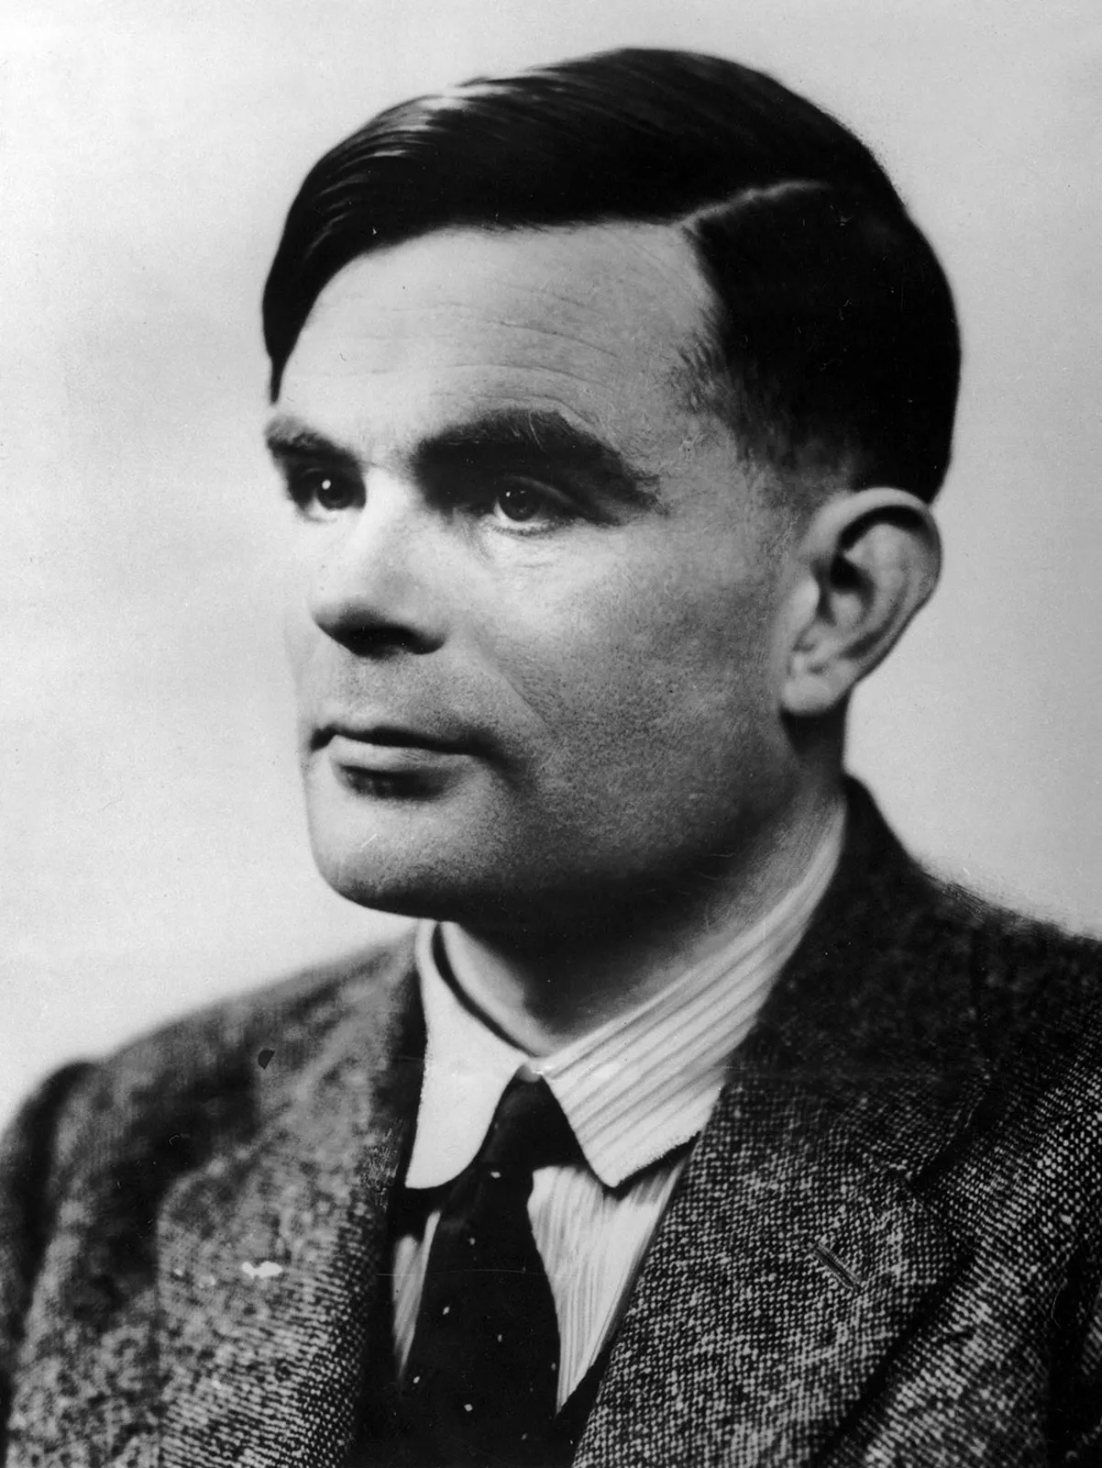
\includegraphics[scale=.4]{images/Alan.png}
    \caption{Alan Turing}
\end{figure}

\section*{Introduction}
Alan Turing was a brilliant British mathematician, cryptologist, and computer scientist
who made revolutionary contributions to any field he touched.
He is famously known as the father of computer science or father of the first modern computer.
His work on the Turing machine, which is a theoretical machine that can compute anything 
that is computable, is considered to be the foundation of computer science.
In mathematics he made many contributions to the theory of computation, the theory of numbers, and the theory of games. 
All of these skills were used during World War II to help save the lives of many people.
Even to this day, his work is still used in many fields of computer science and mathematics.
In this paper, we will look at his life and his contributions to the world.

\section*{Early Life}
Alan Turing was born on June 23, 1912 in London, England to Julius Mathison Turing and Ethel Sara Turing.
He was the second child of his parents, and had an older brother John and a younger sister Joan.
His father was a senior colonial administrator of the British Empire
and his mother was the daughter of the chief engineer of Madras railway.
He first attended St. Michael's Church of England School in London
at six years old, and then went to Sherborne School in Dorset at the age of thirteen.
He was a very bright student that was very interested in mathematics and science.
His teachers at Sherborne School disapproved of his interest in science and mathematics,
and was more focused on his studies in Latin and Greek.
Although being disapproved of, he still continued to study mathematics and science on his own
and learned many things independently.
Without formal tutelage in calculus, he was able to learn it on his own and was able to solve 
advanced calculus problems by himself. At the age of sixteen, he was learning both
Albert Einstein and Isaac Newton's theories very quickly and soon was questioning them.
After graduating from Sherborne School, his next academic stop was King's College in Cambridge.

\section*{Academic Career}
Alan Turing was accepted into King's College in Cambridge in 1931 to study mathematics.
He graduated in 1934 with first class honors from his research on probability theory.
In his research, he was able to prove the central limit theorem, which then lead to him
to become a fellow at King's College in 1935.
During his time at King's College, he was able to make many contributions to mathematics.
His most famous paper was ``On Computable Numbers, with an Application to the Entscheidungsproblem,''
published in 1936, which became the foundation of computer science and later in his work on the Turing machine.
The conclusion of his paper was also the same as another paper published by Alonzo Church in 1936.
This lead into Turing moving to Princeton University in 1937 to work with Alonzo Church along with getting his PhD.

\section*{The Entscheidungsproblem}
The Entscheidungsproblem is a problem in mathematics that determines if a given mathematical statement
is true or false. The problem was first posed by David Hilbert and Wilhelm Ackermann in 1928
and posed the question of an effective procedure to determine whether a given mathematical statement or 
problem is provable or not. In 1936, both Alan Turing and Alonzo Church published papers
that proved that the Entscheidungsproblem is undecidable.
They both came to the conclusion that there is no effective procedure or formal 
decision method that can determine whether a given mathematical statement is true or false.
They used examples with both arithmetic and logical systems to show that there is no effective procedure.
This solution caused many mathematicians to lose hope of finding a system 
to simplify methods that anyone could carry out.

\section*{World War II}
Following Turing's work on the Entscheidungsproblem and his time at Princeton University,
he moved back to England to continue his fellowship at King's College.
During this time, World War II began to start and Turing was asked to join the British Government Code and Cypher School.
After the war broke out, Turing, along with select others, moved to the famous headquarters of the British Government's
Code breaking department in Bletchley Park, Buckinghamshire. 
At Bletchley Park, Turing and this select group of people were tasked 
to break the German Enigma code daily, a code that was used by the German military.

\subsection*{The Enigma Code}
The Enigma code was a code that was used by the German military to send messages to each other.
If the code could be broken, it would allow the British to know what the Germans were planning at every
moment, and would allow them to manuever their troops accordingly.
The Enigma code was created in 1918 by Arthur Scherbius, a German engineer, and was initally used for 
commercial purposes. The Enigma code could have over 150 million different combinations, and was
considered to be unbreakable. During the war, there was already a machine that was able to break the Enigma code,
called the Bomba, created by the Polish mathematician Marian Rejewski. The Bomba however was rendered useless
when the Germans changed the Enigma code in 1940. The Germans changed the code to make it more difficult to break,
and having it have different operating procedures. 

\subsection*{Turing's Contributions}
Turing and his team were tasked to break this new code.
Having tried decoding the Enigma code by hand, Turing found that it was too difficult and inefficient to do so.
Turing devised a plan to create a machine that would be able to break the Enigma code, even with the new changes.
Turing and his team would tirelessly work on the machine from 1939 to 1940 to finally create a machine that could break
the Enigma code called the Bombe. The Bombe was built from Turings research on the Entscheidungsproblem and 
deriving a ``Turing machine.'' The machine worked great and was able to translate
2 messages every minute, 24/7, leading to more than 80,000 messages being translated a month.
Due to this, Turing was awarded the OBE (Order of the British Empire) in 1946 for his work on the Bombe and code breaking.

\begin{figure}[h]
    \centering
    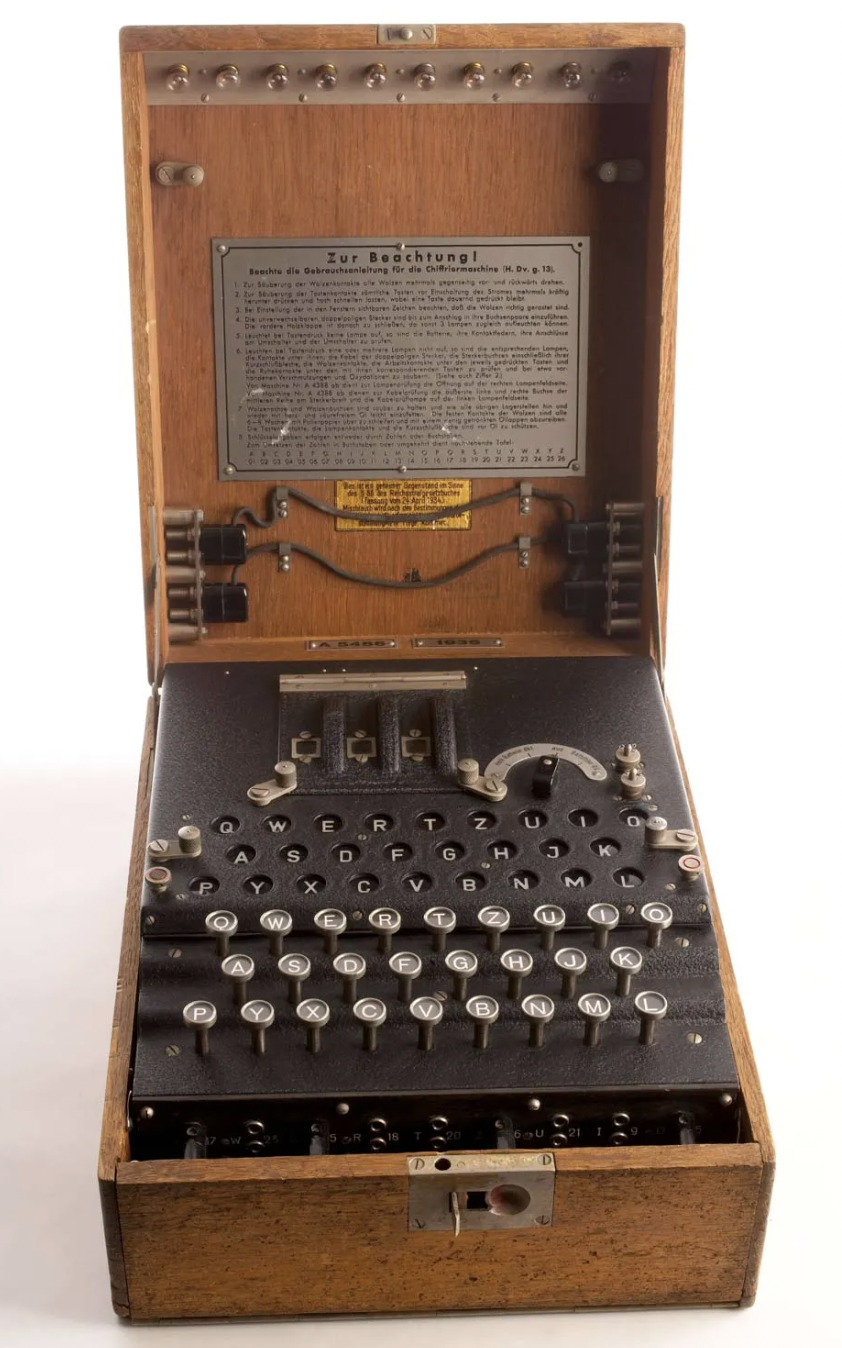
\includegraphics[scale=.3]{images/Enigma.png}
    \caption{A Enigma Machine}
\end{figure}

\section*{The Turing Machine}
The Turing machine is a theoretical machine that is more like a mathematical model.
This machine was based off of the work that Turing did on the Entscheidungsproblem.
It was first derived as a mathematical model to find if a mathematical statement from a
formal axiomatic system is true or false. Turing was able to use this model to create a 
model that breaks down the process of computation into a series of logical steps.
The machine would do discrete steps of computation, and would be able to do any computation
that is computable. Turing was able to use this model to create a machine that could break the Enigma code.
The end result would be a solution to a given problem unless it is a problem that is undecidable
where the machine would not be able to find a solution and run forever causing a halting problem.

\begin{figure}[h]
    \centering
    \includegraphics[scale=.3]{images/Bombe.png}
    \caption{Bombe}
\end{figure}

\section*{After the War}
After the war, Turing continued his work on the Turing machine and joined
the National Physical Laboratory in Teddington, Middlesex. 
In the National Physical Laboratory, Turing worked on the ACE project, which was a project
to create a computer that could be used for scientific calculations. Turing was able to create
a prototype of the ACE computer, but was not able to finish it due to the difficulties of the project.
NPL sadly was beaten to the punch by the Royal Society Computing Machine Laboratory at the University of Manchester
who created the first digital stored-program computer, the Manchester Baby. Frusturated with the lack of progress
and delays in NPL, Turing left the NPL in 1948 to join the Computing Machine Laboratory as a deputy director.
With Turing's diverse knowledge and experince from his work on the Turing machine and the Bombe, Turing was able
to help the Computing Machine Laboratory improve their development on all of their projects.
Turing also created the first programming manual and helped with the first commercial computer, the Ferranti Mark I.

\section*{The Turing Test}
During his time at the Computing Machine Laboratory, Turing was able to create a test that would
determine if a machine could think like a human. Turing named this test the Turing Test.
The test was created to determine if a machine could think like a human by having a human
interact with a machine and a human. The human would not know which one was the machine
and which one was the human. If the human could not tell which one was the machine and which one was the human,
then the machine would be considered to be able to think like a human. 

\section*{Final Years}
In 1951, Turing was elected a fellow of the Royal Society of London.
From that point onwards, Turing focused on his work to create a artificial intelligence machine.
Sadly, Turing was convicted of "gross indecency" in 1952.
Being convicted of this crime, Turing was forced to undergo hormone treatment to chemically castrate him.
This however slowly made Turing's health deteriorate and he was forced to take his own life in 1954.
To this day, Turing is still considered to be one of the greatest minds of the 20th century.
His work on the Turing machine and the Bombe are still used today in the field of computer science and 
has been improved upon by many other great minds.
Due to his accomplishments and treatment he was formally apologized by both the British government and the Queen in 2013.
To this day Turings work still resonates with many people and is still used to this day.

\nocite{*}
\bibliographystyle{plain}
\bibliography{sources.bib}


\end{document}